% vim:ts=4:sw=4
% Copyright (c) 2014 Casper Ti. Vector
% Public domain.

\chapter{高速公路关键路段识别模型}
		对于交通运输\parencite{NewmanBasic}、水利传输\parencite{test}、能源和通信等基础设施系统,在遭遇自然灾害或者人为灾害时,会对整个系统的性能造成显著的影响,带来重大的经济损失。所以在发生事故或者自然灾害的时候,维护这些网络的完整性至关重要。

		灾难管理是一个多阶段的过程,从防灾减灾和准备,着眼于长期消除或降低风险的措施,延伸到灾后 响应、恢复与重构。投资 基础设施系统在缓解中起着至关重要的作用 活动,它可以增强链接的稳定性。但是,将所有的路段稳定性都增强到坚不可摧,在管理人员看来是十分浪费的,甚至会达到负担不起预算的水平。本章节主要研究如何在有限的资源下,找到可以最大化网络通行效率关键路段进行管理。即将资源投放到高速公路路段集合的一个关键子集,同时尽量增加高速公路的通行效率,以达到宏观层面增强路网稳定性的目的,实现事故前的预防,事故后的快速恢复。

		这一章主要研究的是如何对高速公路关键路段挖掘问题进行建模,以及围绕着安徽、山西、北京的收费站车辆数据,进行建模之后的求解。

		\section{模型定义}
			高速公路具有成网性,给定一个有向图$G=\{V,E\}$,其中V代表收费站(节点)的集合;E表示边的集合,也就是高速公路中路段的集合。对于通过高速公路出行的车辆,定义O为车辆的出发节点,D作为车辆的目标节点。定义$P_e$(0<$P_e$<1)为路段的损毁率,这个概率通过历史上的高速公路路段损毁事件得到,同时可以随着交通管理者对路段进行管理、布置资源而减小。定义管理者的决策向量y=\{$y_1$,$y_2$,$\cdots$,$y_n$\},y是一个n维向量,每一维$y_i$的数值取0或1,1表示这条路段属于关键路段,管理者会进行维护和投资管理,改善路段状况;0表示非关键路段,暂时不关注。因为每一条路段都有一定的概率损毁,所以用$C_{e_i}$来表示第i个路段是否损毁,当$C_{e_i}$等于1时,路段保持完好,当$C_{e_i}$等于0时,路段因为事故损毁。定义$\bm{c}$=\{$C_{e_1}$,$C_{e_2}$,$\cdots$,$C_{e_n}$\},c表示路网的某一种拓扑结构,$\bm{C}$表示路网的所有拓扑结构的集合。对于行驶在高速公路上的车辆,定义车辆的出行时间为$X_i$,这个出行时间由车辆的路径选择、出行时途径路径的车流密度决定。定义当高速公路路段断裂严重,车辆无法抵达目的地时,车辆的出行时间定为常量M。M的大小在一定程度上代表了路网连通性的权重,M越大,高速网络的连通性就越重要。为了更好的求解目标函数,在此提出两个假设:

			1)路段之间的损毁概率相互独立:假设处于静态模型下,所有路段在下一时刻都有一定的概率损毁,同时这个损毁不会影响到其他路段的损毁率。在传统研究网络可靠性的相关文献中[3],都是基于这个假设做的研究。

			2)M>Max($X_i$):M必须要大于连通路网中的最大出行代价。当车辆在路段中找不到一条可以抵达终点的路径时,我们默认对于该车辆来说,他此次出行的代价要绝对大于路段仍然连通情况下的任意时间。即默认断裂对路网造成的影响一定大于路段仍然连通的情况。


			根据高速公路的历史事故数据,通过结构分析和统计调查[23],确定路段损毁的概率,作为本文的先验概率。高速公路建设管理者可以通过在高速路段上建立基础设施,投放人力资源等方式管理路段,增强路段的稳定性。假设路段$e$以概率$P_e$损毁,以概率$(1-P_e)$保持完好。基于路段的损毁率,我们可以计算路网拓扑结构概率矩阵Z:

		\[\begin{array}{*{20}{c}}
		{C_{{e_1}}^1}&{C_{{e_2}}^1}& \cdots &{C_{{e_n}}^1}&{{P^1}}\\
		{C_{{e_1}}^2}&{C_{{e_2}}^2}& \cdots &{C_{{e_n}}^2}&{{P^2}}\\
		 \vdots & \vdots & \ddots & \vdots & \vdots \\
		{C_{{e_1}}^m}&{C_{{e_2}}^m}& \cdots &{C_{{e_n}}^m}&{{P^m}}
		\end{array}\]


		矩阵中,$C_{{e_i}}$表示第i条路段的状态,0表示遭遇事故,已经损毁,1表示完好无损;对于每一行来说,前n项$C^j = \{{C_{{e_1}}^j},{C_{{e_2}}^j},\cdots,{C_{{e_n}}^j}\}$表示路网的拓扑结构,全0表示全部路段断裂,路网瘫痪;全1表示路网完全连通。第n+1项$P^j \ = \ \prod\limits_{i = 1}^n {({P_{{e_i}}}C_{{e_i}}^j + (1 - {P_{{e_i}}})} (1 - C_{{e_i}}^j))$表示高速公路网络拓扑变成这个拓扑结构的概率。在交通管理者选取关键路段,并进行一定的决策、处理后,路段的损毁概率发生变化,进而路网拓扑结构概率矩阵Z也会发生变化。

		在此提出关键路段挖掘模型:

		\begin{equation}
		L(\bm{y}) = -E(T(\bm{c}|\bm{y} ))
		\label{eq1}
		\end{equation}

		其中,$T(\bm{c}|\bm{y} )$:

		\begin{equation}
		T(\bm{y} ) = P(K|\bm{c})\sum\limits_{k \in K} {{X_k}} 
		\label{eq2}
		\end{equation}

		$\bm{y} $表示管理者想要投资维护的路段,$T(\bm{c}|\bm{y} )$表示当关键路段集合为$\bm{y}$,路网拓扑结构为c的时候,高速公路的整体通行时间。式\ref{eq1}中对时间的期望取负,转化为通行效率。模型的研究目标是探究如何选取关键路段,对这些关键路段增加投入,使得在同样的预算情况下,整个路网的通行效率得到最大的提升。结合式\ref{eq1},式\ref{eq2},得到展开式:

		\begin{equation}
		Max(L(\bm{y})) = -Mi{n_{\bm{y} }}\sum\limits_{\bm{c} \in C} {P(\bm{c}|\bm{y} )} P(K|\bm{c})\sum\limits_{k \in K} {{X_k}} 
		\label{eq3}
		\end{equation}

		式中$\bm{y} $表示关键路段集合,假设高速公路网络的路段数量为n,则$\bm{y} $为n维向量,对于$\bm{y} $的第i个维度,如果值为0,则表示第i个路段不是关键路段,反之表示第i个路段是关键路段;$\bm{c}$表示路网的拓扑结构,C是高速公路网络所有拓扑结构的集合;${P(\bm{c}|\bm{y} )}$表示当关键路段集合为$\bm{y} $时,高速路网的拓扑结构为$\bm{c}$的概率;k表示第k个车辆的出行路径,K表示所有车辆的出行路径集合;$P(K|\bm{c})$表示当路网拓扑结构为$\bm{c}$时,高速公路车辆出行路径集合为K的概率;${{X_k}}$表示当车辆的行驶路径为k时,车辆的行驶时间。

		\section{基于博弈的用户出行方式}
			当用户出行$O-D$矩阵与路网拓扑结构$c$确定时,所有用户的总出行时间期望就已经确定了。

		\section{子模性分析}
			\subsection{子模性定义}
			次模函数(submodular function)是一种具有“边际效应递减”效应的函数,即对于一个集合函数,如果$S \subseteq V$,那么在V中增加一个元素所增加的收益要小于等于在S的子集中增加一个元素所增加的收益。形式化表述就是:对于函数f而言,若$A \subseteq B \subseteq V$,且$\varepsilon  \in V - B$,则$f(A \cup \{ \varepsilon \} ) - f(A) \ge f(B \cup \{ \varepsilon \} ) - f(B)$;或者若$A \subseteq \Omega,B \subseteq \Omega$,则$f(A) + f(B) \ge f(A\mathop  \cup \nolimits B) + f(A\mathop  \cap \nolimits B)$;或者对于任意$X \subseteq \Omega,x_1,x_2 \in \Omega$,下面的式子一定成立:$f(X \cup {x_1}) + f(X \cup {x_2}) \ge f(X \cup {x_1},{x_2}) + f(X)$。满足这三个条件中的任意一个,函数f即满足子模性。

			\subsection{子模性证明}
				假设$\varepsilon$是某一条路段,$\bm{y}$和$\bm{Y}$都是关键路段的集合,$\bm{\Omega}$是关键路段集合的全集空间,$\bm{y} \subseteq \bm{Y} \subseteq \bm{\Omega}$。$\varepsilon \in \Omega \ - \ Y$。$\{y \ + \ \varepsilon\}$表示对于关键路段集合$y$,将$\varepsilon$作为新的关键路段加入,形成新的关键路段集合。

				定义:
				\begin{equation}
				I\ =\ L(\bm{y+\varepsilon})-L(\bm{y})-(L(\bm{Y+ \varepsilon}) - L(\bm{Y}))
				\label{eq3}
				\end{equation}

				不妨假设$Y = y\ +\ \varepsilon_2$,公式$\ref{eq3}$转化为:$I\ =\ L(\bm{y+\varepsilon_1})-L(\bm{y})-(L(\bm{y+ \varepsilon_1+\varepsilon_2}) - L(\bm{y+\varepsilon_2}))$

				令$J\ =\ L(\bm{y+\varepsilon_1})-L(\bm{y})$,要证明$I \ge 0$,即证$J$单调非增。

				$J$属于有限离散函数,对$J$进行求导化简[3],得到:$\frac{{dy}}{{dx}} = \sum {(\sum\limits_{{c_1}|y + \varepsilon } {P({c_1})}  - \sum\limits_{{c_2}|y} {P({c_2})} )} {X_k}$。显然${\sum\limits_{{c_1}|y + \varepsilon } {P({c_1})} * X_k}$具有单调非减性,导数恒大于等于0。模型的子模性得到证明

				由于对于具有子模性的模型,贪心求解的精度误差不会超过$\frac{1}{e} * OPT$,所以模型可以用贪心方法近似求解。
		\section{贪心求解}
			贪心算法主要用于简化算法的复杂度,采用一步步获取局部最优解的方式,得到最终解集。在本小节中,遍历n条路段,计算每一条路段被选为关键路段之后对高速公路通行效率的影响,选出影响最大的那条边作为关键路段。不断迭代遍历直到关键路段的数量达到预算:
 
		\begin{algorithm}[h]
        \caption{贪心算法求解模型}  
        \label{tanxin}
        \begin{algorithmic}[1] %每行显示行号  
            \Require 高速车辆O-D数据,高速公路网络拓扑结构,关键路段数量,路段损毁率
            \Ensure 高速公路关键路段集合
            \Function{Greedy}{$ODMatrix,G={V, E},B,P_e$}  
                \State $res\gets 0$  
                \State $Array\gets []$  
                \State $k\gets 0$  
                \State $l\gets 0$  
                \While{$len(Array) \le B$}  
                	\For{$i \in E - Array$}  
                		\If{$L(Array+i)>k$}  
                        	\State $k=L(Array+i)$  
                        	\State $l=i$  
                    	\EndIf
                	\EndFor    
                    \State $res\gets k$
                    \State $Array\gets Array+l$
                \EndWhile  
                \State \Return{$Array$}  
            \EndFunction  
        \end{algorithmic}  
    	\end{algorithm} 

    	为验证贪心算法的效果,在此引入对比方法:

    	算法\ref{meiju}使用枚举方法,获取最优解。从n条路段中,枚举$C_n^B$种情况,计算每一种情况下的高速公路通行效率的变化,从中选取最优解。

    	\begin{algorithm}[!h]
        \caption{枚举} 
        \label{meiju} 
        \begin{algorithmic}[1] %每行显示行号  
            \Require 高速车辆O-D数据,高速公路网络拓扑结构,关键路段数量
            \Ensure 高速公路关键路段集合
            \Function{Enumeration}{$ODMatrix,G={V, E},B,P_e$}  
                \State $res\gets 0$  
                \State $Array\gets []$  
                \State $k\gets 0$ 
                	\For{$l \in \Omega$ \textbf{and} $len(l) \le B$}  
                		\If{$L(l)>k$}  
                        	\State $k=L(l)$  
                        	\State $Array=l$  
                    	\EndIf
                	\EndFor  
                \State \Return{$Array$}  
            \EndFunction  
        \end{algorithmic}  
    	\end{algorithm} 

    	算法\ref{tuopu}利用高速公路网络拓扑结构,抽取关键路段。算法中的Z(i)是计算路段i的中心性函数,该方法引用经典路段中心性来度量关键路段。

    	\begin{algorithm}[!h]
        \caption{拓扑中心性}  
        \label{tuopu}
        \begin{algorithmic}[1] %每行显示行号  
            \Require 高速公路网络拓扑结构,关键路段数量
            \Ensure 高速公路关键路段集合
            \Function{Enumeration}{$ODMatrix,G={V, E},B$}  
                \State $res\gets 0$  
                \State $Array\gets []$  
                \State $k\gets \{\}$ 
                	\For{$i \in E$}  
                		\State $k\gets \{i,Z(i)\}$ 
                	\EndFor  
                \State $SortbyValue(k)$
                \State $Array\gets k[0:B]$
                \State \Return{$Array$}  
            \EndFunction  
        \end{algorithmic}  
    	\end{algorithm} 

    	算法\ref{tongji}基于统计学方法,计算路段重要程度,获取关键路段。式中$f_i$表示路段e的流量。:

    	\begin{algorithm}[!h]
        \caption{统计}  
        \label{tongji}
        \begin{algorithmic}[1] %每行显示行号  
            \Require 高速公路网络拓扑结构,关键路段数量,高速公路路段损毁概率
            \Ensure 高速公路关键路段集合
            \Function{Enumeration}{$G={V, E},B,P_e$}  
                \State $res\gets 0$  
                \State $Array\gets []$  
                \State $k\gets \{\}$ 
                \For{$i \in E$}  
                	\State $k\gets \{i,f_i*P_i\}$
                \EndFor  
                \State $SortbyValue(k)$
                \State $Array\gets k[0:B]$
                \State \Return{$Array$}  
            \EndFunction  
        \end{algorithmic}  
    	\end{algorithm} 


		\section{实验及结果}
		本节针对各种方法在真实的交通数据集中进行实验,通过对比已有的关键路段挖掘方法,评估模型的效果。实验环境为:Windows Server 2008,64GB RAM,Inter(R)Xeon(R) CPU E7-4830 2.13GHz 2.13GHz (2处理器),后续章节的实验均在相同的实验环境下进行。特别地,实验中采用了两个国内高速公路网的数据:安徽省和山西省高速公路网数据。
			\subsection{实验数据}
				本节的实验数据来自于安徽省和山西省的高速公路路网,其中主要的数据为高速路网中车辆的行驶O-D数据。路网中包含142个出口位置和142个入口位置。为了方便研究,将车辆的O-D数据整合为出行O-D矩阵ODMatrix:
				\[\begin{array}{*{20}{c}}
				{{a_{11}}}&{{a_{12}}}& \cdots &{{a_{1n}}}\\
				{{a_{21}}}&{{a_{22}}}& \cdots &{{a_{2n}}}\\
				 \vdots & \vdots & \ddots & \vdots \\
				{{a_{n1}}}&{{a_{n2}}}& \cdots &{{a_{nn}}}
				\end{array}\]

				其中,$a_{ij}$表示以收费站i为起点O,以收费站j为终点D的车辆数量。

				还有高速公路路段损毁概率,这个通过统计历史的路段损毁次数获得,部分数据库已有,部分通过新闻抓取。路段的损毁包括交通事故损毁,重大自然灾害损毁,重大堵车事故等。

			\subsection{实验结果}
				图\ref{fig1:a},\ref{fig1:b}给出了在不同时间区段下,几种方法的最终结果比较。图\ref{fig1:a}是基于2010年10月30日一天的实验结果,纵坐标代表路网整体通行效率(路网整体通行时间取负)的绝对值,横坐标代表一天内的不同时间段,本实验中以1小时为一个时间段,采样八个时间点[0-1,3-4,6-7,9-10,12-13,15-16,18-19,21-22]。由图\ref{fig1:a}可以发现,在整体上贪心算法明显优于统计算法,同时统计算法又比直接基于高速公路拓扑结构获取关键路段有效,原因是高速公路整体网络结构比较简单,路网拓扑结构的某些性质体现的不明显。在不同的时间段,高速公路的流量在不断变化,不同方法的效果之间的差异大小也在变化,在高速公路车流最少的午夜,几种方法差异达到最小,从六点开始,到流量最高的中午,三种方法之间的差异逐渐增大,这体现了高速公路流量对关键路段选取后效果的影响,流量越大,关键路段维护后造成的效益越大。图\ref{fig1:b}是基于从2010年10月10日开始,到2010年10月16日为止一周数据的实验,纵坐标和图\ref{fig1:a}一样,表示网络整体的通行时间。纵坐标以一天为一个时间段,从当天0点采样到当天24点,采样七天(从周日到下一个周六)。可以发现,在以一整天的O-D矩阵为数据集进行研究时,不同天之间的路网通行效率变化较小,不同方法之间的差异也趋于平稳。这证明了高速公路具有一定的稳定性和规律性,可以通过研究某个月的数据,获取关键路段,同时这些关键路段在宏观角度来看具有普适性。



				%插入图片
				%\5个收费站的情况下
				\begin{figure}[h]
				\begin{minipage}{0.5\linewidth}
					\centering
					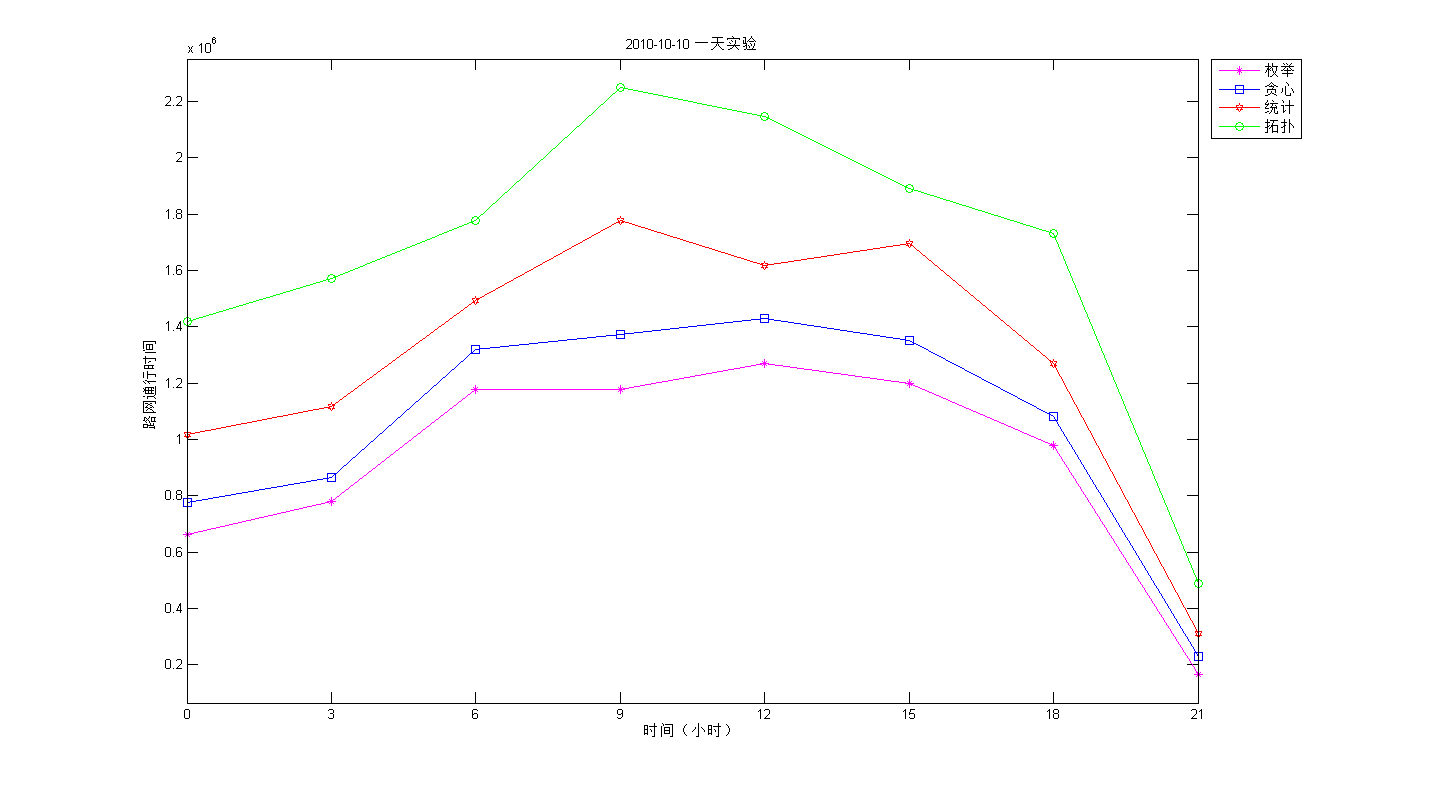
\includegraphics[width=3.0in]{picture/one_day_5}
					\caption{关键路段挖掘:以1h为区间}
					\label{fig1:a}
				\end{minipage}%
				\begin{minipage}{0.5\linewidth}
					\centering
					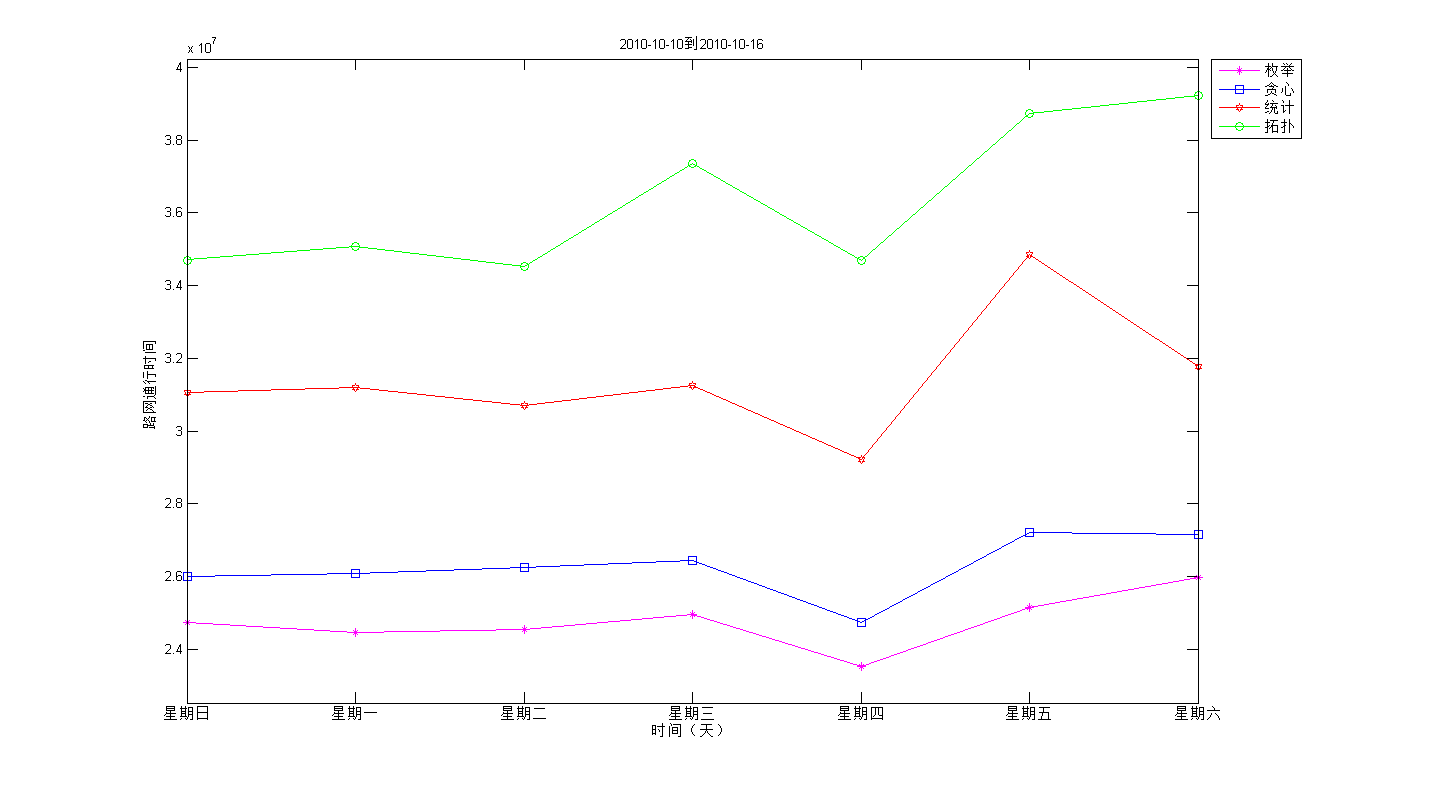
\includegraphics[width=3.0in]{picture/one_week_5}
					\caption{关键路段挖掘:以1d为区间}
					\label{fig1:b}
				\end{minipage}
				\end{figure}

				表\ref{tab:5}给出了不同方法求得的路网通行效率。表格中的数值是$L(\bm{y})$的绝对值(路网整体通行时间),可以看出贪心算法最接近最优解,而且误差在可接受范围内。

				\begin{table}[h]
				\centering
				\begin{tabular}{|c|c|c|c|c|}
				\hline
				\hline
				   &   枚举 &   贪心 &   统计 &   拓扑 \\
				\hline
				  一天 &  926030.06 & 1053575.26 & 1287439.55 & 1660243.55 \\
				\hline
				  一周 &  21674024.80 & 22989458.02 & 27510044.42 & 31790488.20 \\
				\hline
				\end{tabular}
				\caption{算法结果集}
				\label{tab:5}
				\end{table} 



				图\ref{fig2}给出了关键路段在路网中的分布图,图\ref{fig2}$(a)$是用贪心算法求得的关键路段集合,图\ref{fig2}$(b)$是高速公路统计方法获得的路段集合。图\ref{fig2}$(c)$是基于枚举所得的最优解集,图\ref{fig2}$(d)$是基于路网拓扑结构选取的关键路段集合。图\ref{fig2}$(a)$中颜色的变化和粗细的变化表示路段在贪心求解过程中,路段被选择的顺序;图\ref{fig2}$(b)$中颜色的变化表示路段的重要程度。对比两图可以发现,直观上重要的点(承载流量较大的路段,事故多发路段等)并不一定在路网中属于关键节点,需要经过一些计算才能求出;直接枚举的路段集合与贪心算法求得的路段集合十分接近,平均有80\%以上的相似度,而统计和度中心性方法求得的关键节点和枚举方法差距较大。

						%插入图片
				%\10个收费站的情况下
				\begin{figure}
				%\begin{tabular}{cc}   
				\begin{minipage}{0.48\linewidth}
				  \centerline{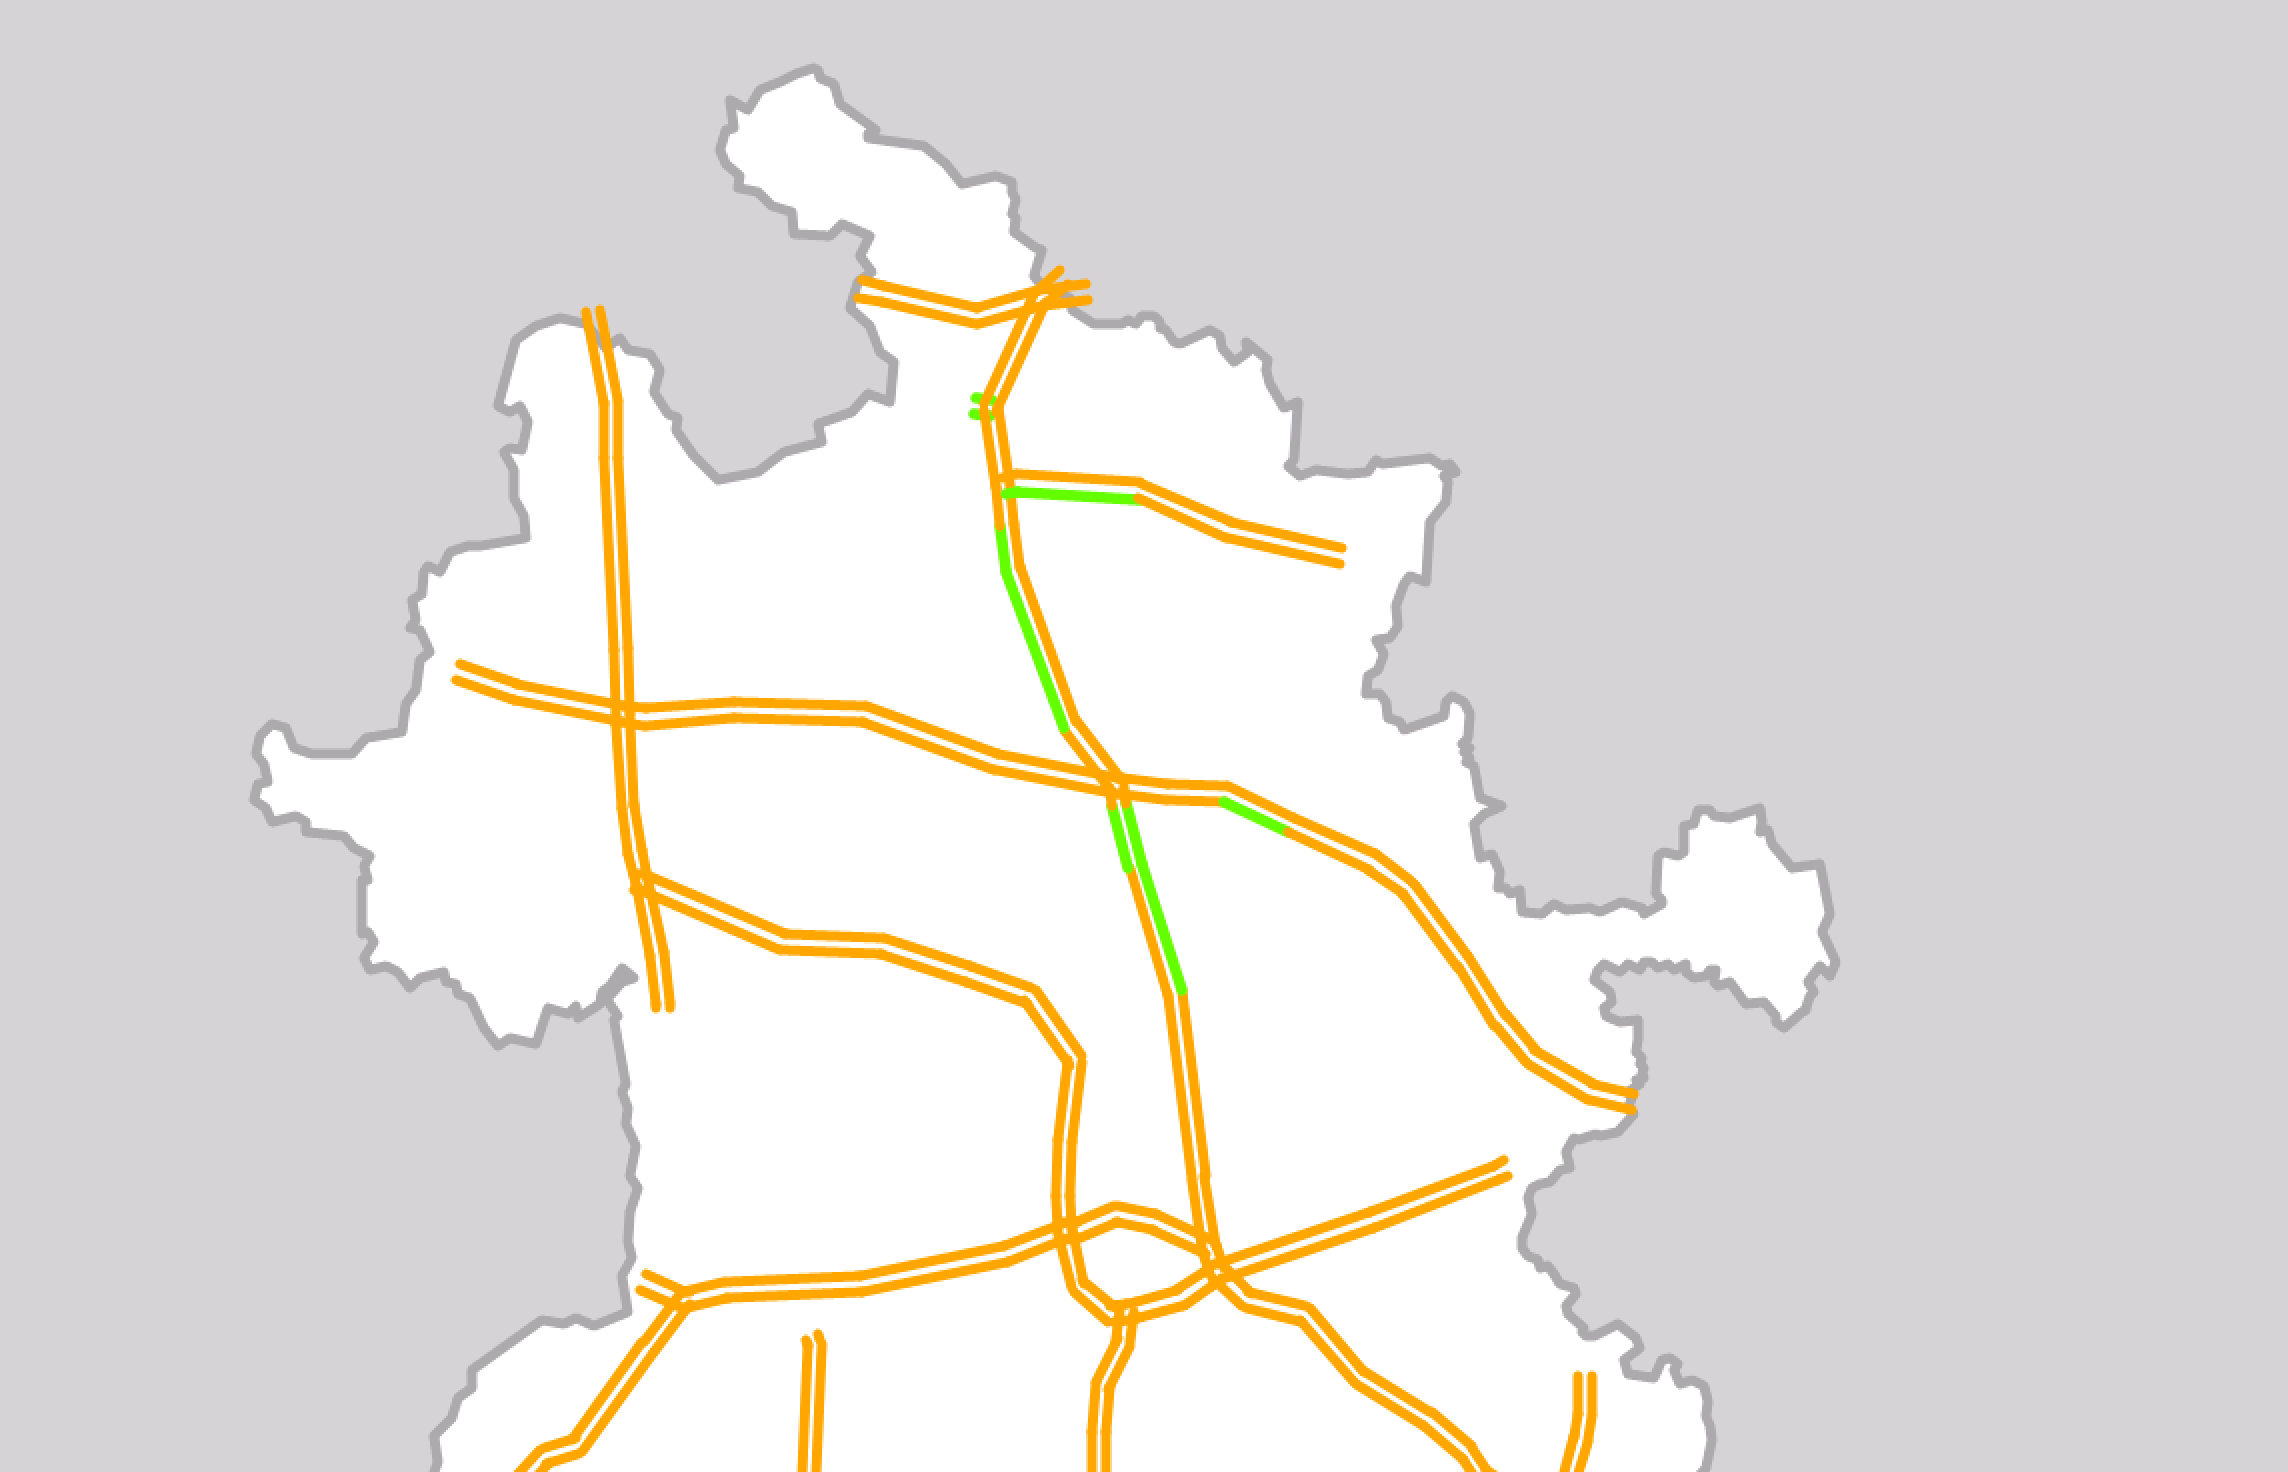
\includegraphics[width=3.0in]{picture/tanxin}}
				  \centerline{(a) 贪心算法关键路段}
				\end{minipage}
				\hfill
				\begin{minipage}{.48\linewidth}
				  \centerline{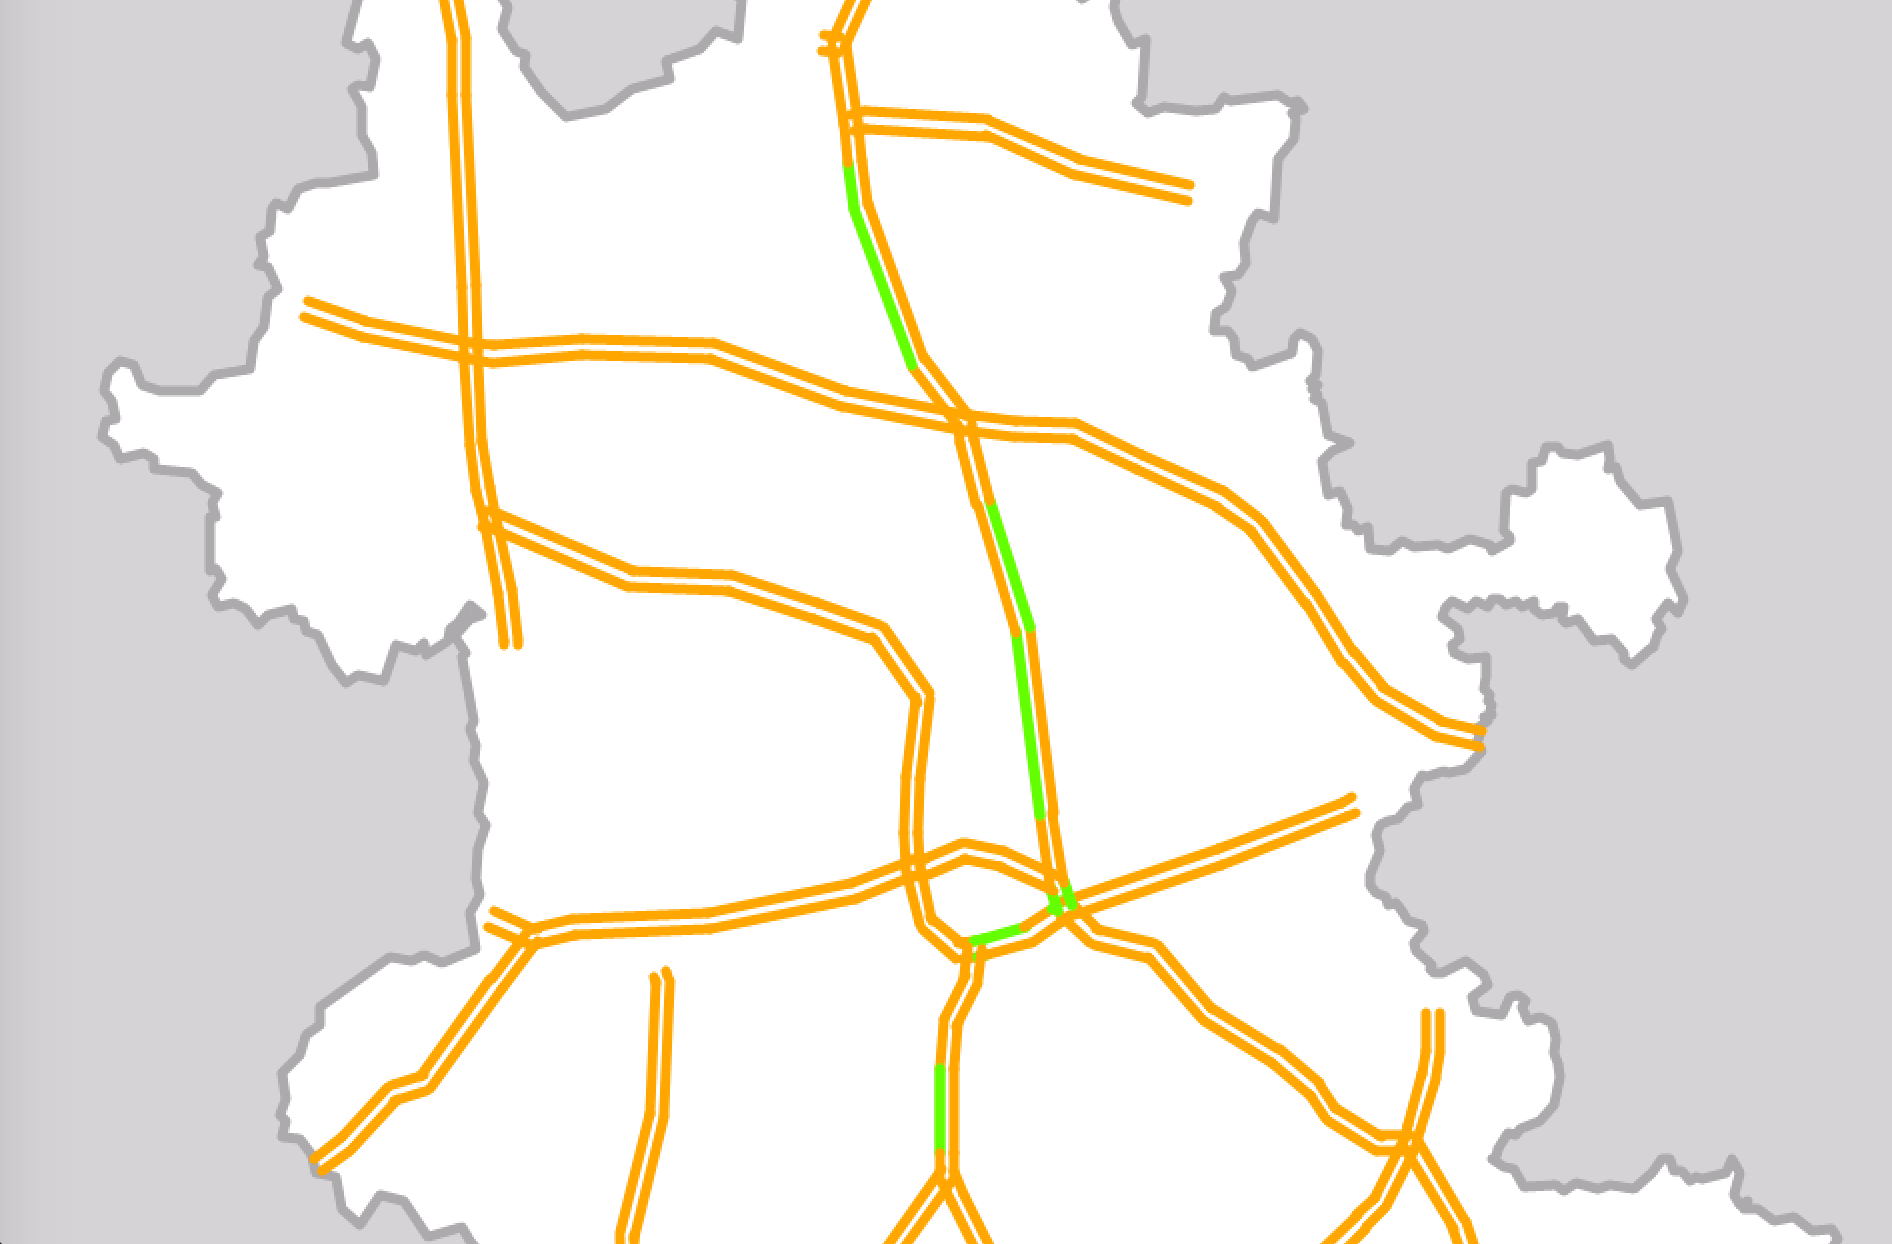
\includegraphics[width=3.0in]{picture/hotsection}}
				  \centerline{(b) 统计获得关键路段}
				\end{minipage}
				\vfill
				\begin{minipage}{0.48\linewidth}
				  \centerline{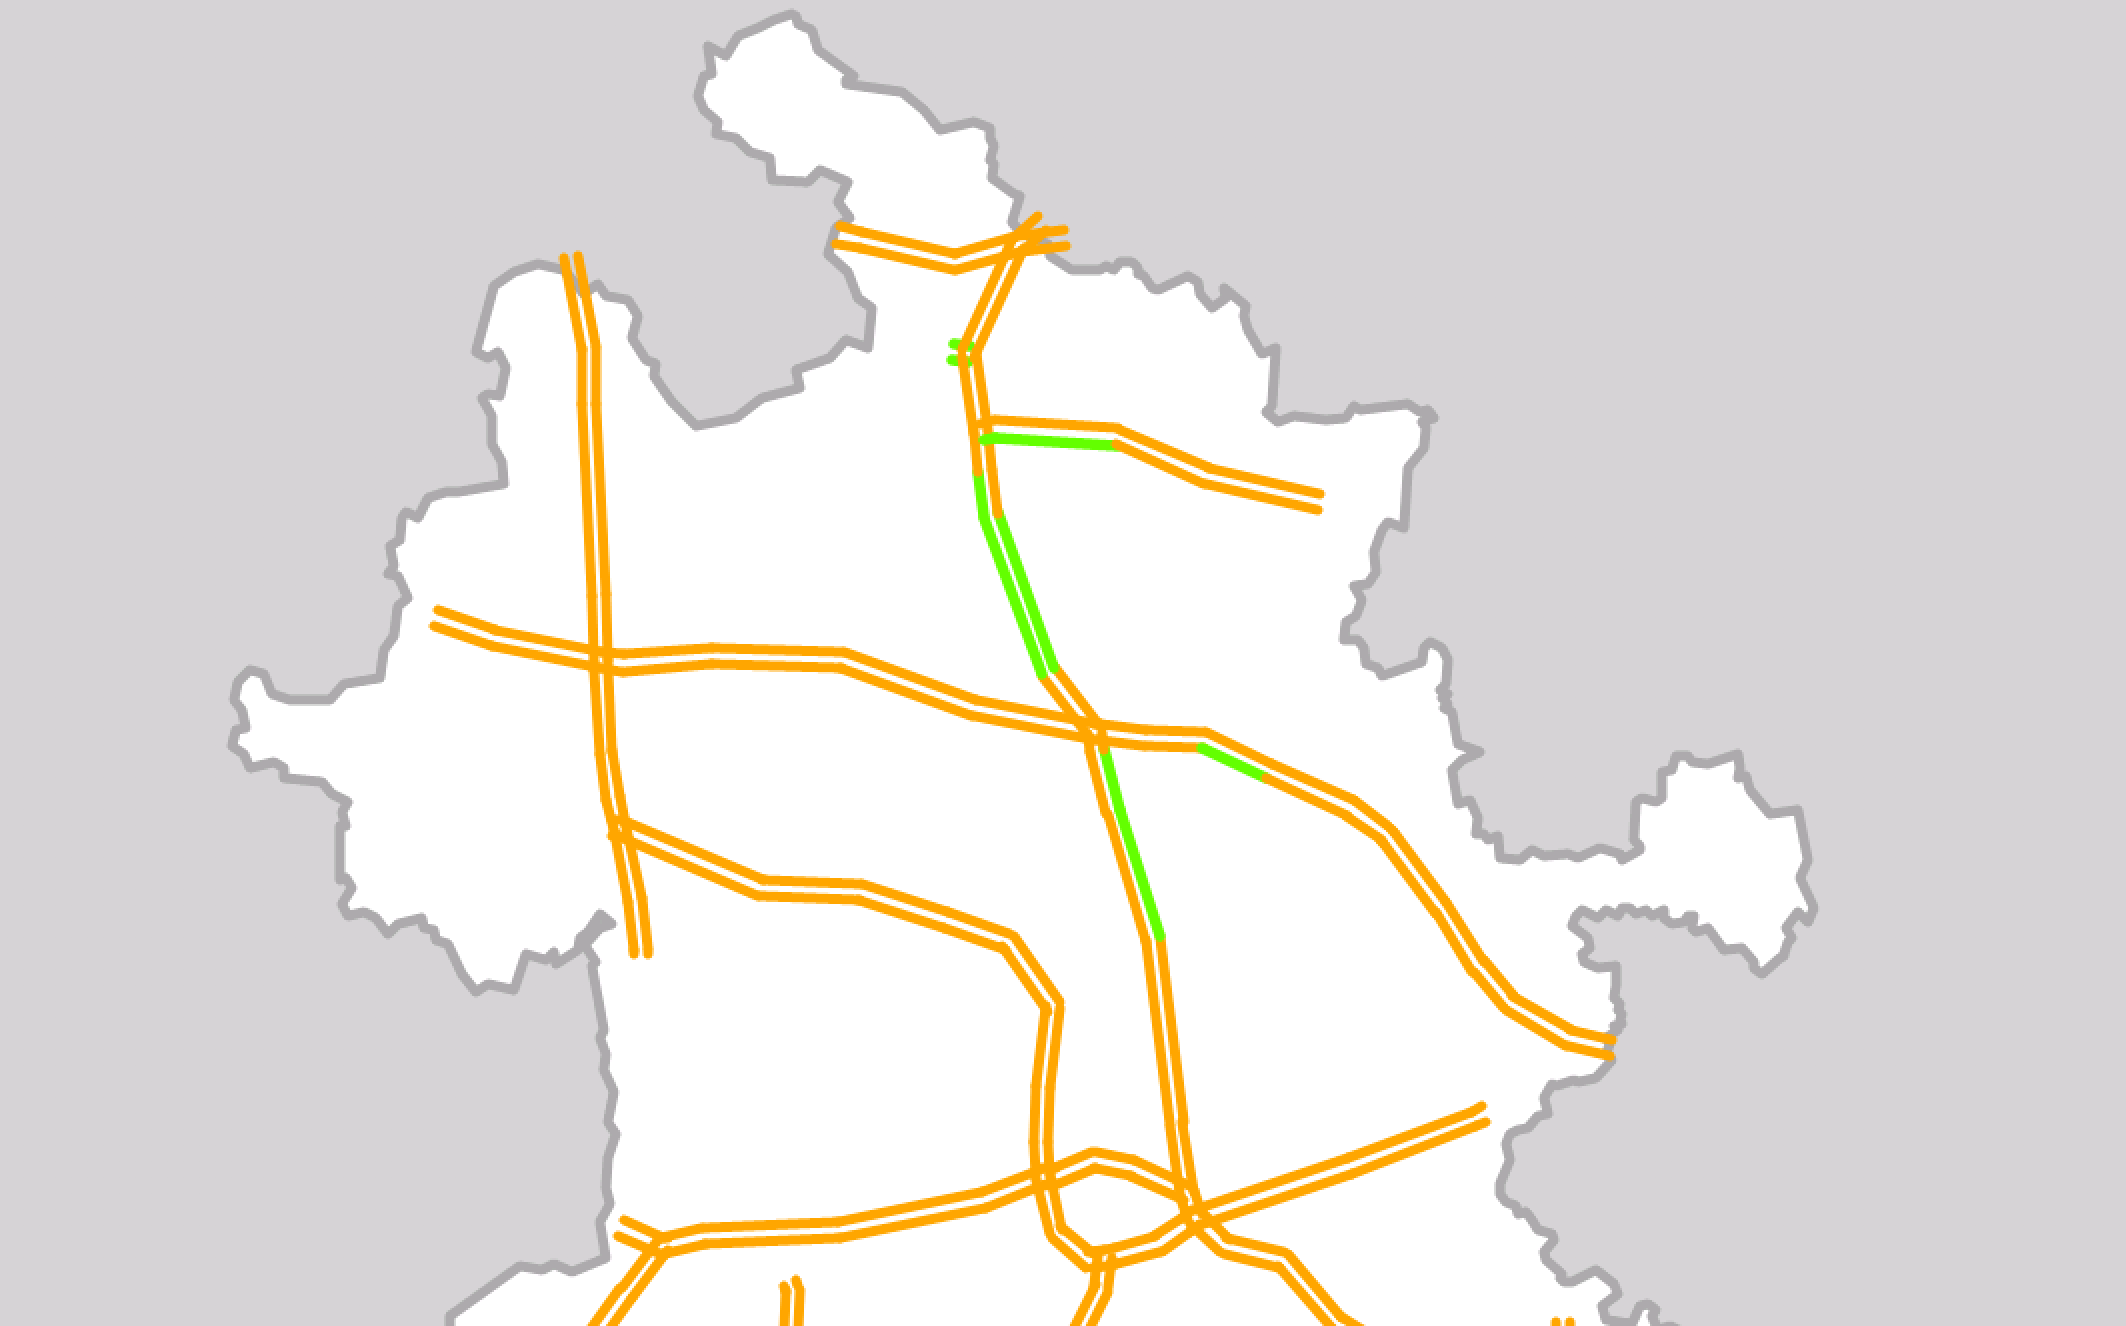
\includegraphics[width=3.0in]{picture/meiju}}
				  \centerline{(c) 枚举获得最优解}
				\end{minipage}
				\hfill
				\begin{minipage}{0.48\linewidth}
				  \centerline{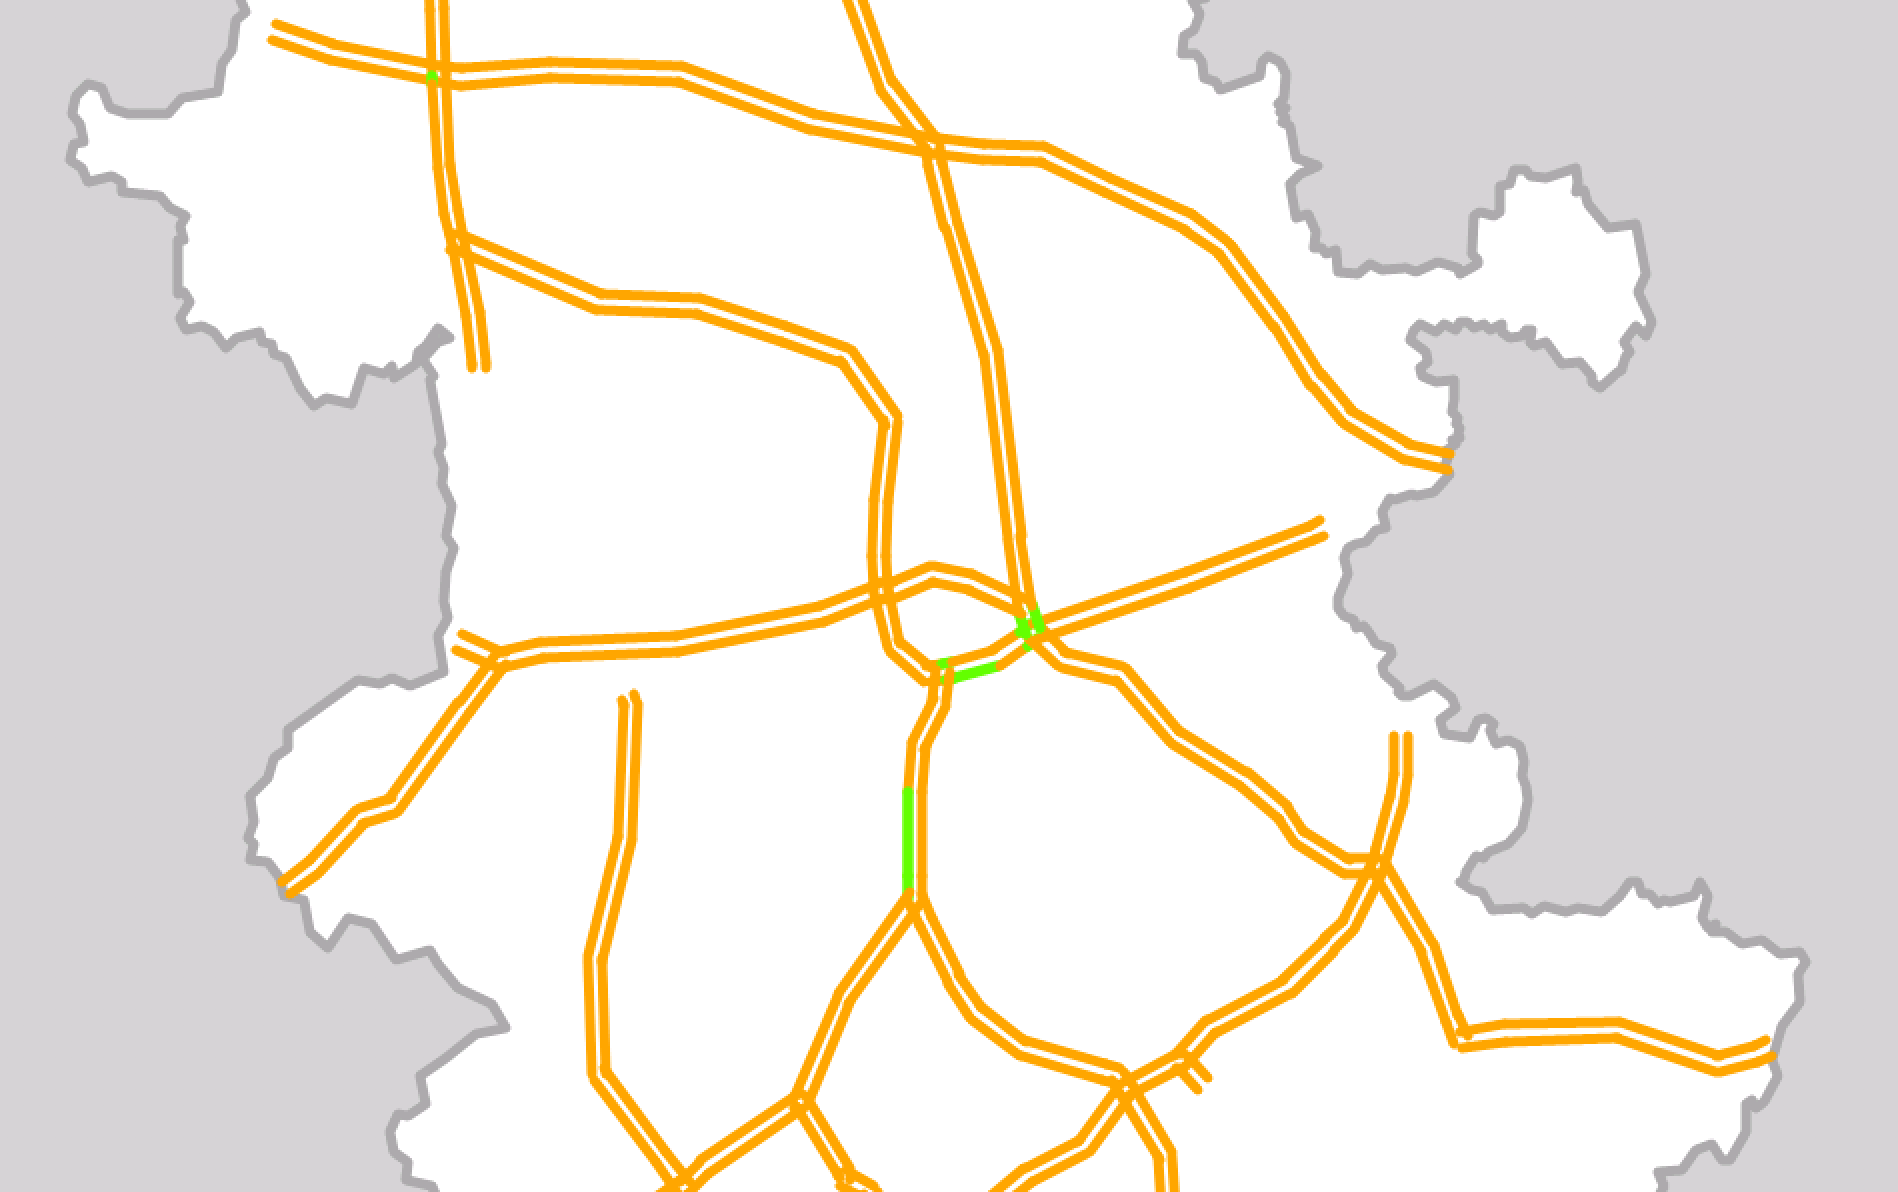
\includegraphics[width=3.0in]{picture/degree}}
				  \centerline{(d) 基于拓扑结构的关键路段}
				\end{minipage}
				%\end{tabular}
				\caption{不同方法求得的关键路段结果图}
				\label{fig2}
				\end{figure}

				在实验过程中,我们还发现当时间区间缩短到1h时,高速公路网络中的关键路段具有随着时间和流量变化而变化的特性。图\ref{duibi1}是凌晨3点时的高速公路关键路段集合,图\ref{duibi2}是早上九点时的高速公路关键节点集合。这一发现证明了高速公路的关键路段具有动态变化特性,他不是一成不变的,而是会随着整个路网的流量的变化而变化。


				\begin{figure}[h]
				\begin{minipage}{0.5\linewidth}
					\centering
					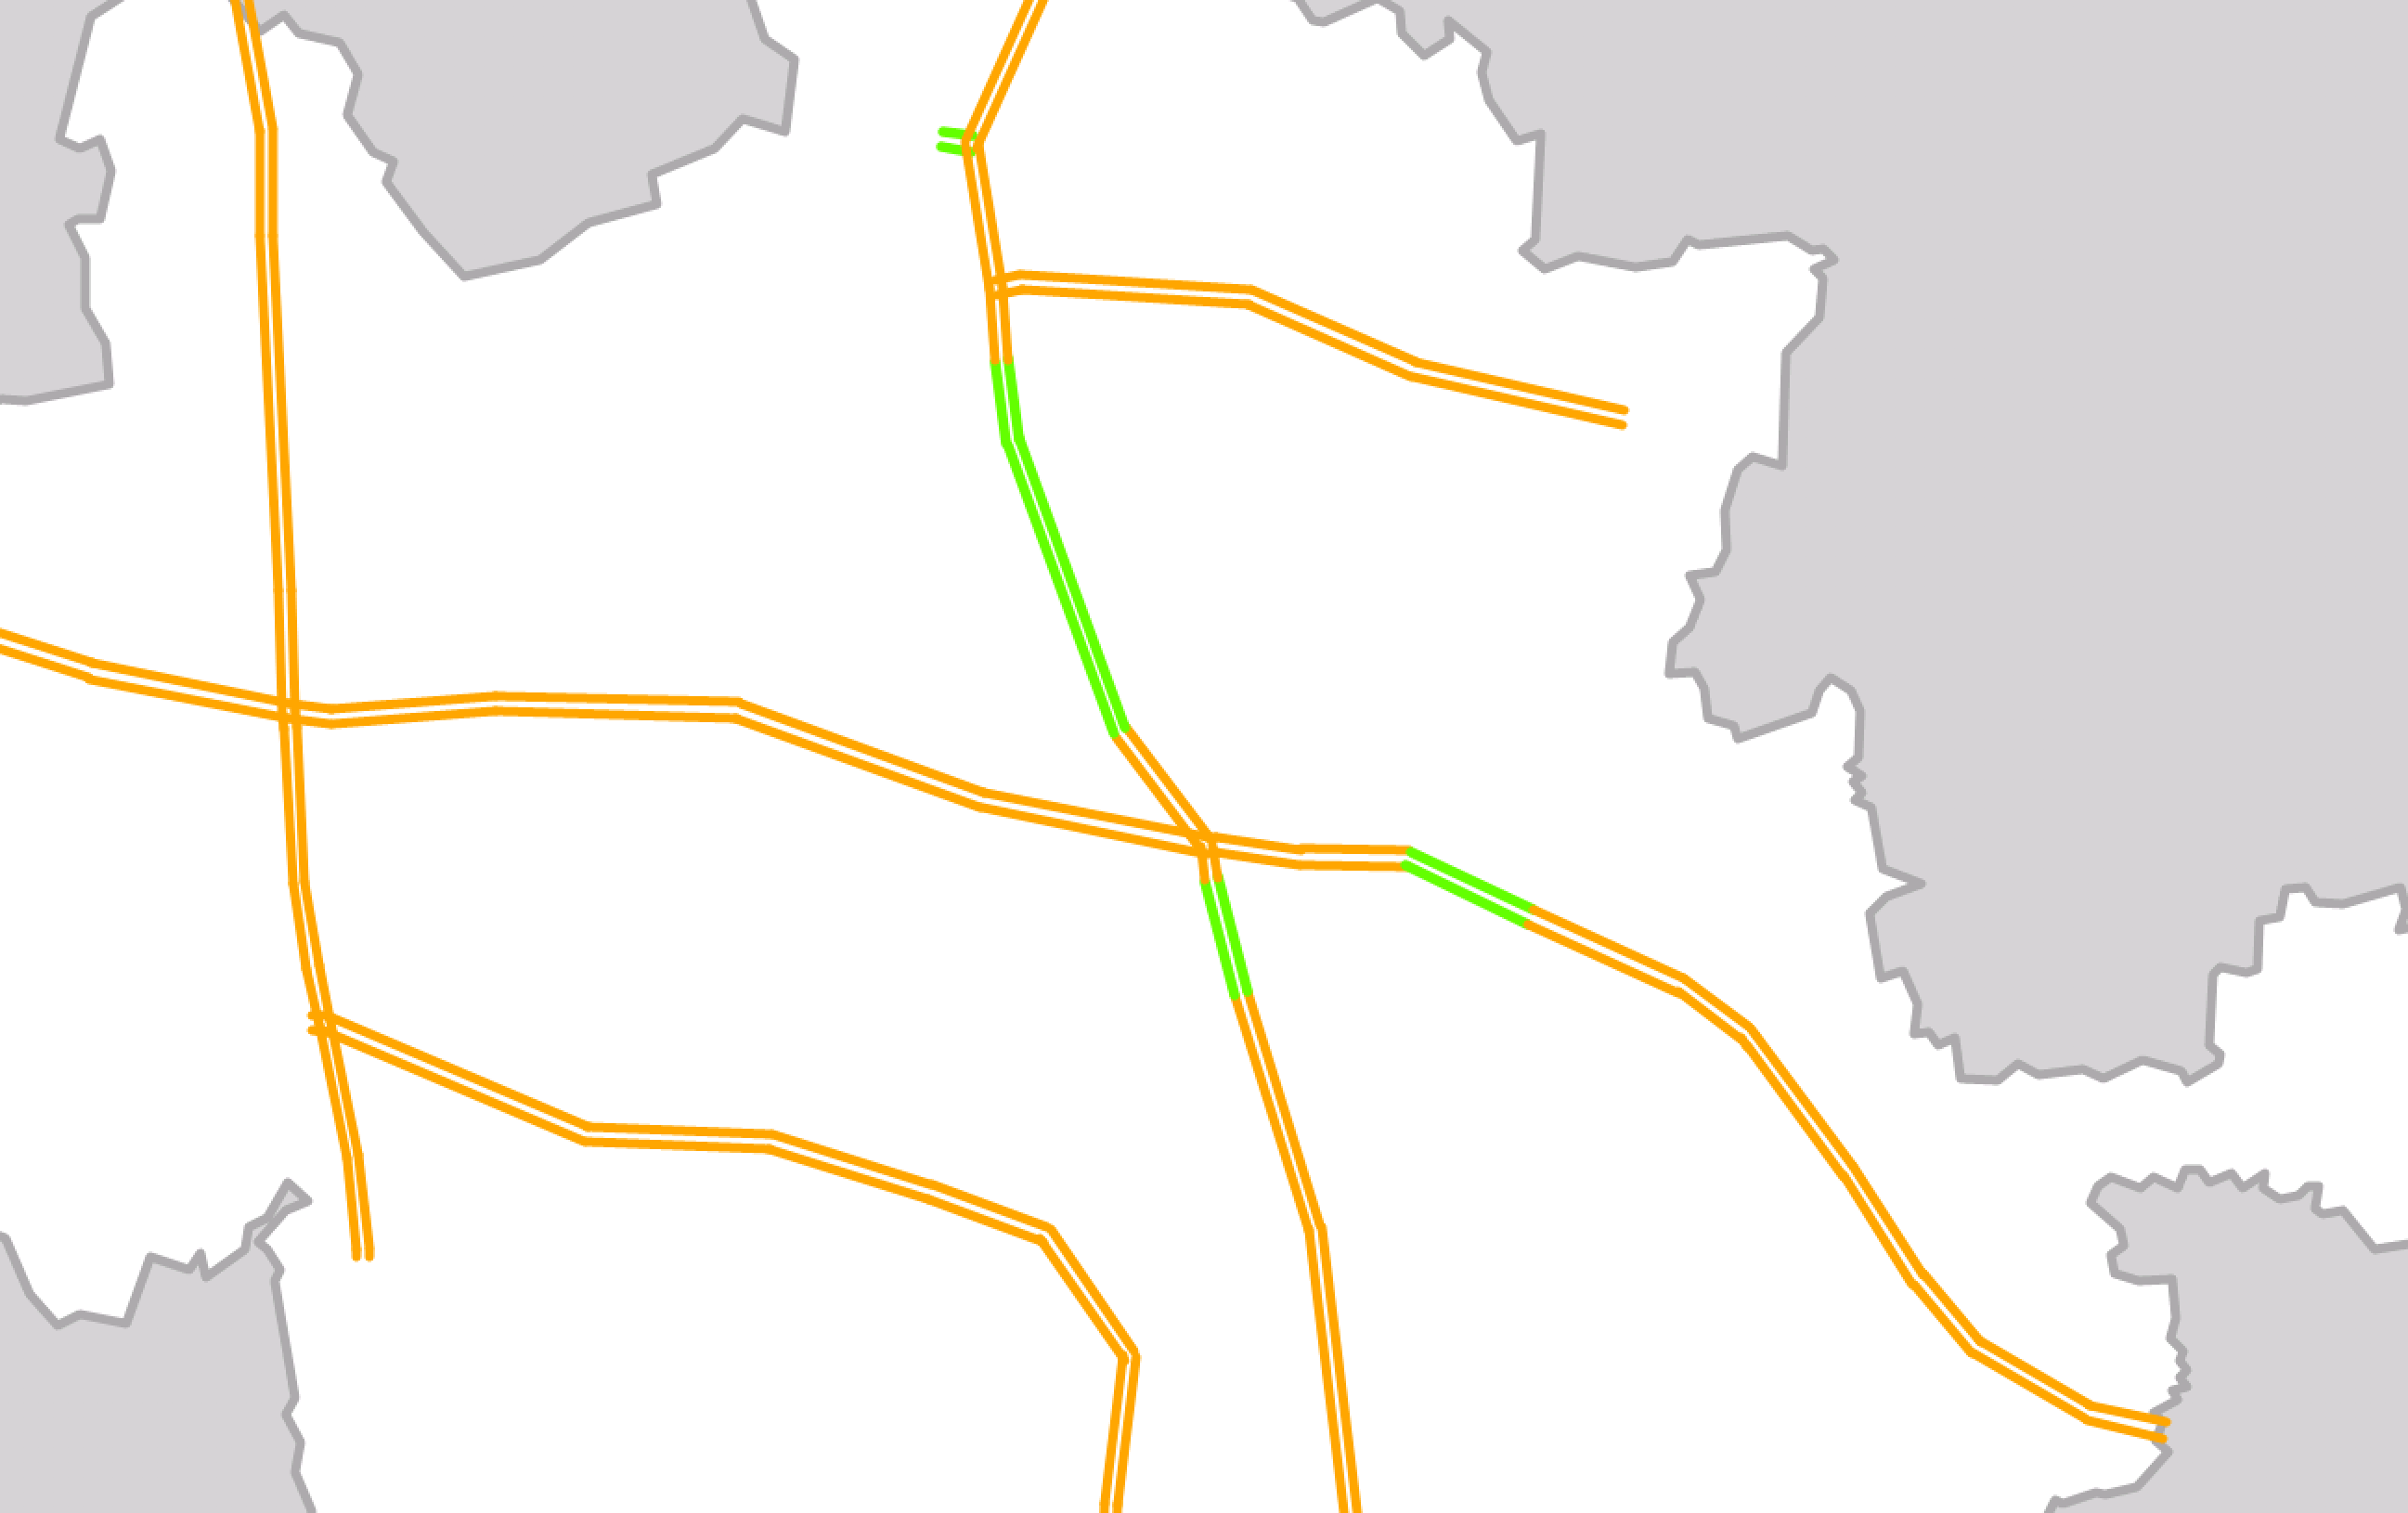
\includegraphics[width=3.0in]{picture/duibi1}
					\caption{关键路段挖掘:03:00}
					\label{duibi1}
				\end{minipage}%
				\begin{minipage}{0.5\linewidth}
					\centering
					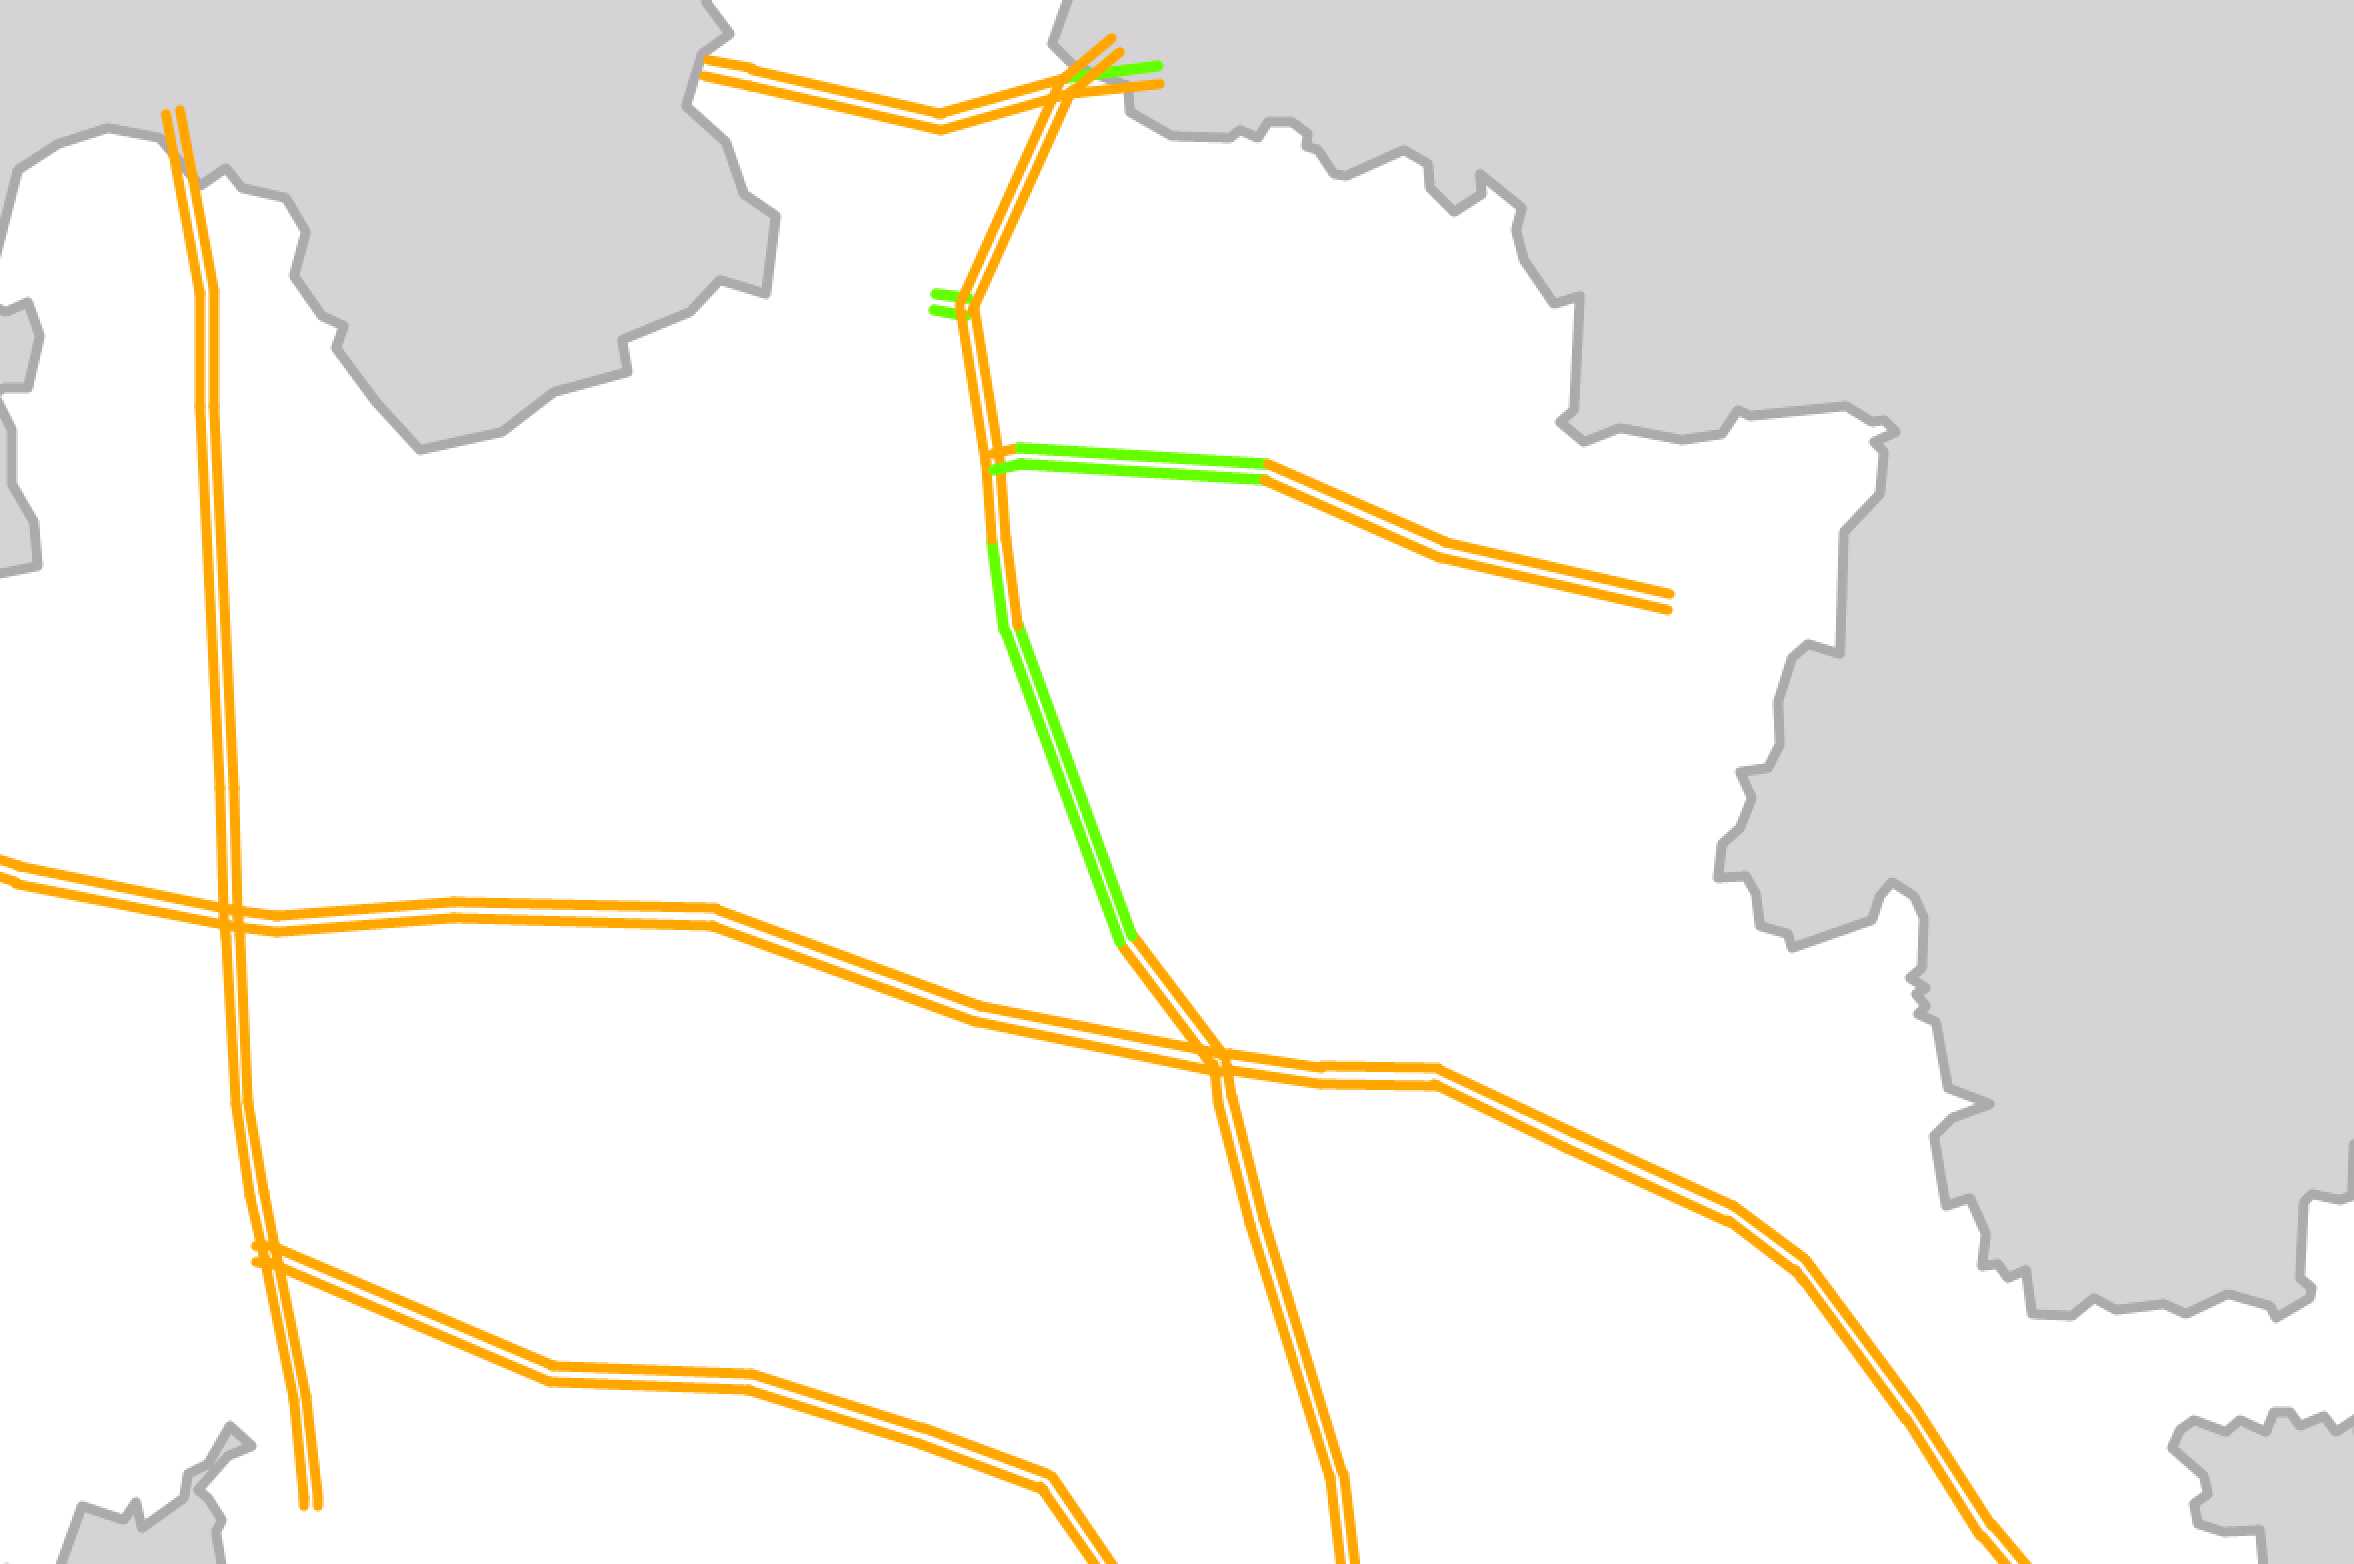
\includegraphics[width=3.0in]{picture/duibi2}
					\caption{关键路段挖掘:09:00}
					\label{duibi2}
				\end{minipage}
				\end{figure}

			\subsection{时间复杂度分析}
				基于暴力枚举方法的时间复杂度:$O({n^B}*{2^n})$

				基于贪心算法的时间复杂度:$O(n*B*{2^n})$

				基于统计路段重要性方法的时间复杂度:$O(n*\log (n))$

				基于路网拓扑结构方法的时间复杂度:$O(n*\log (n))$

				其中,后两个方法可以用大根堆将时间复杂度优化到O(n)。
				实验时间如表\ref{table1}所示,第一行代表实验的方法,第一列代表实验数据的范围,表格内的数值是实验的平均运行时间。

				\begin{table}[h]
				\centering
				\begin{tabular}{|c|c|c|c|c|}
				\hline
				\hline
				   &   枚举 &   贪心 &   统计 &   拓扑 \\
				\hline
				  一小时 &   1day &   30min &   1min &   1min \\
				\hline
				  一天 &   6day &   2h &   2min &   1min \\
				\hline
				  一周 &   7day &   3h &   5min &   1min \\
				\hline
				  一月 &   7day &   3h &   8min &   1min \\
				\hline
				\end{tabular}
				\caption{不同算法的运行时间}
				\label{table1}
				\end{table} 

				由表格可以看出,在以一个省为数据集的基础上,枚举方法已经处于一种较大的时间复杂度;贪心算法在一定程度上解决了算法过慢的情况,并且在精度上有一定的保证,可以应用于静态路网关键节点识别问题,但是对于动态实时应用仍旧不够;基于统计领域的路段重要性排序方法、基于路网拓扑结构的关键节点挖掘方法虽然在时间上运行极快,但是在精度上打不到要求。

		\section{本章小结}
			本章提出了一种面向高速公路网络的关键节点挖掘模型,同目前高速公路关键路段已有的挖掘方法相比,该方法的优势是结合高速公路的特性,考虑高速公路上的车流流量、路段事故率,从宏观角度提出一个整体的优化模型。针对上述模型,本章分析了模型的子模性,单调性。特别的,本文的实验中使用枚举方法,获取高速公路中的最优解。结果表明该模型的贪心算法解集可以很好地逼近数据中真实解,并且在时间复杂度上有了规模性的优化,证明了贪心算法的可行性。然而,即使贪心算法可以在一定规模上优化整体的时间复杂度,并且可以在实际应用中起到不错的作用,但是这是基于目前研究的场景是静态关键路段挖掘模型,以及高速公路只有部分路段产生过阻断重大事故的情况下达成的。当任务环境更为复杂时(扩大到全国高速公路网络),当管理者需要更加快速得到实时反馈的时候,上述方法收到算法计算规模的约束,无法达到预期的效果。下一章将针对高速公路的O-D特点,提出相应的解决手段。





			
